%%%%%%%%%%%%%%%%%%%%%%%%%%%%%%%%%%%%
% Slide options
%%%%%%%%%%%%%%%%%%%%%%%%%%%%%%%%%%%%

% Option 1: Slides with solutions

\documentclass[slidestop,compress,mathserif]{beamer}
\newcommand{\soln}[1]{\textit{#1}}
\newcommand{\solnGr}[1]{#1}

% Option 2: Handouts without solutions

%\documentclass[11pt,containsverbatim,handout]{beamer}
%\usepackage{pgfpages}
%\pgfpagesuselayout{4 on 1}[letterpaper,landscape,border shrink=5mm]
%\newcommand{\soln}[1]{ }
%\newcommand{\solnGr}{ }

%%%%%%%%%%%%%%%%%%%%%%%%%%%%%%%%%%%%
% Style
%%%%%%%%%%%%%%%%%%%%%%%%%%%%%%%%%%%%

\def\chp7@path{../../Chp 7}
\input{../../lec_style.tex}


%%%%%%%%%%%%%%%%%%%%%%%%%%%%%%%%%%%%
% Preamble
%%%%%%%%%%%%%%%%%%%%%%%%%%%%%%%%%%%%

\title[Lecture 24]{MA213: Lecture 24}
\subtitle{Module 4: Inference}
\author{OpenIntro Statistics, 4th Edition}
\institute{$\:$ \\ {\footnotesize Based on slides developed by Mine \c{C}etinkaya-Rundel of OpenIntro. \\
The slides may be copied, edited, and/or shared via the \webLink{http://creativecommons.org/licenses/by-sa/3.0/us/}{CC BY-SA license.} \\
Some images may be included under fair use guidelines (educational purposes).}}
\date{}


%%%%%%%%%%%%%%%%%%%%%%%%%%%%%%%%%%%%
% Begin document
%%%%%%%%%%%%%%%%%%%%%%%%%%%%%%%%%%%%

\begin{document}


%%%%%%%%%%%%%%%%%%%%%%%%%%%%%%%%%%%%
% Title page
%%%%%%%%%%%%%%%%%%%%%%%%%%%%%%%%%%%%

{
\addtocounter{framenumber}{-1} 
{\removepagenumbers 
\usebackgroundtemplate{\includegraphics[width=\paperwidth]{../../OpenIntro_Grid_4_3-01.jpg}}
\begin{frame}

\hfill \includegraphics[width=20mm]{../../oiLogo_highres}

\titlepage

\end{frame}
}
}


%%%%%%%%%%%%%%%%%%%%%%%%%%%%%%%%%%%%
% Recap/Agenda 
%%%%%%%%%%%%%%%%%%%%%%%%%%%%%%%%%%%%
% TODO better formatting
\begin{frame}
    \frametitle{Module 4: Inference}
    \begin{itemize}
        \item \hl{Previously: }Testing for independence in two-way tables (Chapter 6.4)
        \item \hl{This time: }One-sample means with the $t$-distribution (Chapter 7.1)
        \item \hl{Reading: }Chapter 7.2 for next time
        \item \hl{Deadlines/Announcements: }HW 4.1 due today
    \end{itemize}
    
\end{frame}
%%%%%%%%%%%%%%%%%%%%%%%%%%%%%%%%%%%%
% Sections
%%%%%%%%%%%%%%%%%%%%%%%%%%%%%%%%%%%%

%%%%%%%%%%%%%%%%%%%%%%%%%%%%%%%%%%%%


\section{One-sample means with the \texorpdfstring{$t$}{t} distribution}

%%%%%%%%%%%%%%%%%%%%%%%%%%%%%%%%%%%%


\begin{frame}
\frametitle{Guinness Quality Control: The Origin of the $t$-test}

\dq{William Sealy Gosset, working at the Guinness Brewery in the early 1900s, wanted to ensure the quality of stout. He would take a small sample of batches and measure a quality metric, (e.g. alcohol content). Suppose the target mean for alcohol content is 4.5\% ABV (percent alcohol by volume). Below is a sample of 8 batches.}

{\scriptsize
\begin{center}
\begin{tabular}{r|c}
Batch & Alcohol Content (\% ABV) \\
\hline
1 & 4.8 \\
2 & 4.6 \\
3 & 4.7 \\
4 & 4.5 \\
5 & 4.9 \\
6 & 4.6 \\
7 & 4.8 \\
8 & 4.4 \\
\end{tabular}
\end{center}
}

\vfill
\rule{2.5cm}{0.25pt} \\
{\tiny Inspired by the original work of W.S. Gosset ("Student") at Guinness Brewery.}

\end{frame}

%%%%%%%%%%%%%%%%%%%%%%%%%%%%%%%%%%%


\begin{frame}
\frametitle{Guinness Quality Control: Framing the Question}

\begin{itemize}
\item We want to investigate if the mean alcohol content of Guinness stout batches differs from the target value of 4.5\% ABV.
\pause
\item One approach is to take a small sample of batches and compare the sample mean alcohol content to the target.
\pause
\item $H_0:$ The average alcohol content is equal to 4.5\% ABV. \\
$H_A:$ The average alcohol content is different from 4.5\% ABV.
\pause
\end{itemize}

$\:$ \\

\dq{Each row in the data set represents the alcohol content measured from a batch of Guiness stout. Are the batch measurements independent?}

\soln{\pause Yes, if batches are produced independently.}

\end{frame}

%%%%%%%%%%%%%%%%%%%%%%%%%%%%%%%%%%%

\begin{frame}
\frametitle{Hypotheses}

\pq{What are the hypotheses for testing whether the mean alcohol content differs from the target value?}

\begin{enumerate}[(a)]
\item  \mathhl{H_0:} $\mu = 0$ \\
\mathhl{H_A:} $\mu \ne 0$
\solnMult{  \mathhl{H_0:} $\mu = 4.5$ \\
\mathhl{H_A:} $\mu \ne 4.5$}
\item  \mathhl{H_0:} $p = 4.5$ \\
\mathhl{H_A:} $p \ne 4.5$
\end{enumerate}

\end{frame}

%%%%%%%%%%%%%%%%%%%%%%%%%%%%%%%%%%%


\begin{frame}
\frametitle{Conditions}

\begin{itemize}
\item \hl{Independence:} We assume each batch is produced independently.
\pause
\item \hl{Sample size / skew:} $\:$ \\
\pause\twocol{0.75}{0.35}
{
{\tiny
\begin{itemize}
\item The sample distribution does not appear to be extremely skewed, but it's difficult to assess with such a small sample size. For alcohol levels, we might expect scores to be fairly symmetric around the target.
\item We do not know $\sigma$ and $n$ is too small to assume $s$ is a reliable estimate for $\sigma$.
\end{itemize}
}
}
{
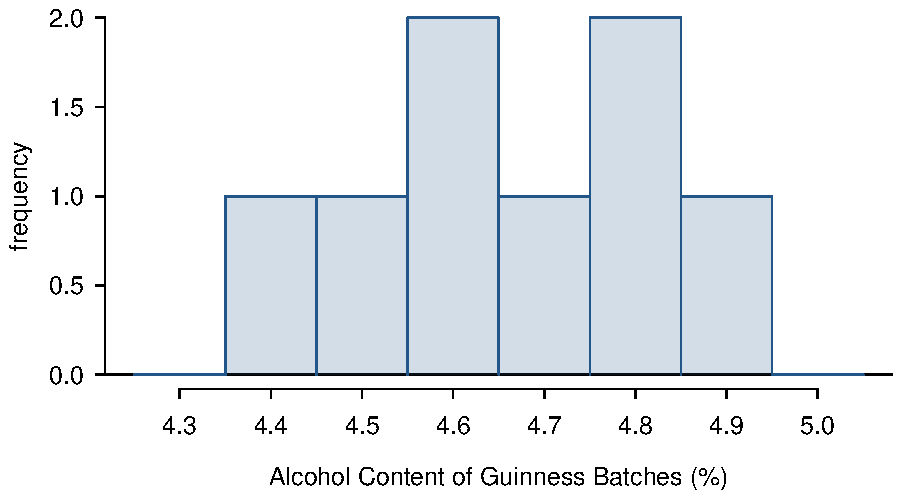
\includegraphics[width=\textwidth]{\chp7@path/7-1_one_t/figures/guiness/guinessHist}
}
\end{itemize}
$\:$ \\
\pause
\dq{So what do we do when the sample size is small?}
\end{frame}

%%%%%%%%%%%%%%%%%%%%%%%%%%%%%%%%%%%

\section{Edfinity Quiz: Intuition check, and what tools do we have for this problem?}

%%%%%%%%%%%%%%%%%%%%%%%%%%%%%%%%%%%

\section{R Demonstration: Try something and see what happens}

%%%%%%%%%%%%%%%%%%%%%%%%%%%%%%%%%%%

\begin{frame}
\frametitle{Review: what purpose does a large sample serve?}

As long as observations are independent, and the population distribution is not extremely skewed, a large sample would ensure that...

\begin{itemize}

\item the sampling distribution of the mean is nearly normal

\item the estimate of the standard error, as $\frac{s}{\sqrt{n}}$, is reliable

\end{itemize}

\end{frame}

%%%%%%%%%%%%%%%%%%%%%%%%%%%%%%%%%%%

\subsection{The normality condition}

%%%%%%%%%%%%%%%%%%%%%%%%%%%%%%%%%%%

\begin{frame}
\frametitle{The normality condition}

\begin{itemize}

\item The CLT, which states that sampling distributions will be nearly normal, holds true for \orange{any} sample size as long as the population distribution is nearly normal.

\pause

\item While this is a helpful special case, it's inherently difficult to verify normality in small data sets.

\pause

\item We should exercise caution when verifying the normality condition for small samples. It is important to not only examine the data but also think about where the data come from. 
\begin{itemize}
\item For example, ask: would I expect this distribution to be symmetric, and am I confident that outliers are rare?
\end{itemize}

\end{itemize}

\end{frame}

%%%%%%%%%%%%%%%%%%%%%%%%%%%%%%%%%%%

\subsection{Introducing the \texorpdfstring{$t$}{t} distribution}

%%%%%%%%%%%%%%%%%%%%%%%%%%%%%%%%%%%

\begin{frame}
\frametitle{The $t$ distribution}

\begin{itemize}

\item When the population standard deviation is unknown (almost always), the uncertainty of the standard error estimate is addressed by using a new distribution: the \hl{$t$ distribution}.

\pause

\item This distribution also has a bell shape, but its tails are \hl{thicker} than the normal model's.

\pause

\item Therefore observations are more likely to fall beyond two SDs from the mean than under the normal distribution.

\pause

\item Extra thick tails are helpful for resolving our problem with a less reliable estimate the standard error (since $n$ is small)

\end{itemize}

\begin{center}
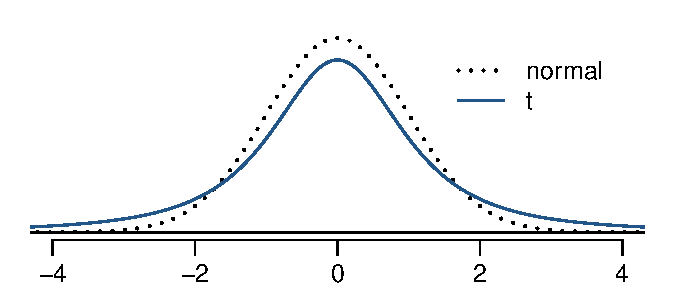
\includegraphics[width=0.5\textwidth]{\chp7@path/7-1_one_t/figures/tDistCompareToNormalDist/tDistCompareToNormalDist}
\end{center}

\end{frame}

%%%%%%%%%%%%%%%%%%%%%%%%%%%%%%%%%%%

\begin{frame}
\frametitle{The $t$ distribution (cont.)}

\begin{itemize}

\item Always centered at zero, like the standard normal ($z$) distribution.

\item Has a single parameter: \hl{degrees of freedom} (\mathhl{df}).

\end{itemize}

\begin{center}
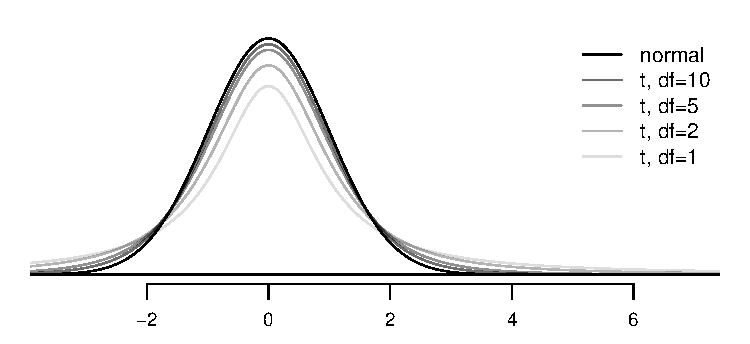
\includegraphics[width=0.8\textwidth]{\chp7@path/7-1_one_t/figures/tDistConvergeToNormalDist/tDistConvergeToNormalDist}
\end{center}

\pause

\dq{What happens to shape of the $t$ distribution as $df$ increases?}

\soln{\pause Approaches normal.}

\end{frame}

%%%%%%%%%%%%%%%%%%%%%%%%%%%%%%%%%%%

\subsection{Evaluating hypotheses using the \texorpdfstring{$t$}{t} distribution}

%%%%%%%%%%%%%%%%%%%%%%%%%%%%%%%%%%%


\section{R Demonstration: Try with \texorpdfstring{$t$}{t} distribution}

%%%%%%%%%%%%%%%%%%%%%%%%%%%%%%%%%%%

\begin{frame}
\frametitle{Back to Guinness: Sample Statistics}

\begin{itemize}
\item Sample mean ($\bar{x}$): 4.66
\item Sample standard deviation ($s$): 0.17
\item Sample size ($n$): 8
\end{itemize}

\begin{align*}
\orange{$\bar{x} = 4.66$} \\
\orange{s = 0.17} \\
\orange{n = 8}
\end{align*}

\end{frame}

%%%%%%%%%%%%%%%%%%%%%%%%%%%%%%%%%%%


\begin{frame}
\frametitle{Finding the test statistic}

\formula{Test statistic for inference on a small sample mean}
{The test statistic for inference on a small sample ($n < 50$) mean is the $T$ statistic with $df = n - 1$.
\[ T_{df} = \frac{\text{point estimate} - \text{null value}}{SE} \]}

\pause

\vspace{-0.5cm}

\hl{in context...}
\begin{eqnarray*}
point~estimate &=& \bar{x} = 4.66 \\
\pause
SE &=& \frac{s}{\sqrt{n}} = \frac{0.17}{\sqrt{8}} = 0.060 \\
\pause
T &=& \frac{4.66 - 4.5}{0.060} = 2.73 \\
\pause
df &=& 8 - 1 = 7
\end{eqnarray*}

\vspace{-0.25cm}

\Note{Null value is 4.5 because in the null hypothesis we set $\mu = 4.5$.}

\end{frame}

%%%%%%%%%%%%%%%%%%%%%%%%%%%%%%%%%%%

\begin{frame}[fragile]
\frametitle{Finding the p-value}

\begin{itemize}
\item The p-value is, once again, calculated as the tail area under the $t$ distribution.
\pause
\item Using R:
\begin{verbatim}
> 2 * pt(2.73, df = 7, lower.tail = FALSE)

# TODO two-sided

[1] 0.523
\end{verbatim}
\pause
\item Visualized below:
\begin{center}
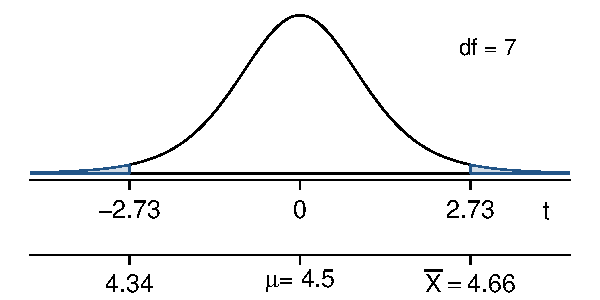
\includegraphics[width=0.7\textwidth]{\chp7@path/7-1_one_t/figures/guiness/guinessPvalue}
\end{center}
\pause
\item Or when these aren't available, we can use a $t$-table.
\end{itemize}
\end{frame}

%%%%%%%%%%%%%%%%%%%%%%%%%%%%%%%%%%%



\begin{frame}
\frametitle{Conclusion of the test}

\dq{What is the conclusion of this hypothesis test?}

\pause

Since the p-value is high, we do not have evidence that the mean alcohol content differs from the target value of 4.5\% ABV.

\end{frame}

%%%%%%%%%%%%%%%%%%%%%%%%%%%%%%%%%%%%

\subsection{Constructing confidence intervals using the \texorpdfstring{$t$}{t} distribution}

%%%%%%%%%%%%%%%%%%%%%%%%%%%%%%%%%%%


\begin{frame}
\frametitle{What is the mean alcohol content?}

\begin{itemize}
\item We did not find evidence that the mean alcohol content differs from the target.
\pause
\item But it would be more interesting to estimate the mean alcohol content itself.
\pause
\item We can use a confidence interval to estimate the mean.
\end{itemize}
\end{frame}

%%%%%%%%%%%%%%%%%%%%%%%%%%%%%%%%%%%

\section{Edfinity Quiz: What is the difference? Try for yourself!}

%%%%%%%%%%%%%%%%%%%%%%%%%%%%%%%%%%%


\begin{frame}
\frametitle{Confidence interval for a small sample mean}

\begin{itemize}
\item Confidence intervals are always of the form
\[ \text{point estimate} \pm {ME} \]
\pause
\item ME is always calculated as the product of a critical value and SE.
\pause
\item Since small sample means follow a $t$ distribution (and not a $z$ distribution), the critical value is a $t^\star$ (as opposed to a $z^\star$).
\[ \text{point estimate} \pm t^{\star} \times SE \]
\end{itemize}
\end{frame}

%%%%%%%%%%%%%%%%%%%%%%%%%%%%%%%%%%%


\begin{frame}[fragile]
\frametitle{Finding the critical $t$ ($t^\star$)}

Using R:
\begin{verbatim}
> qt(p = 0.975, df = 7)

[1] 2.364624
\end{verbatim}
\end{frame}

%%%%%%%%%%%%%%%%%%%%%%%%%%%%%%%%%%%


\begin{frame}
\frametitle{Constructing a CI for a small sample mean}

\pq{Which of the following is the correct calculation of a 95\% confidence interval for the mean alcohol content?}
\[ \bar{x} = 4.46 \qquad s = 0.17 \qquad n = 8 \qquad SE = 0.060 \]

	wocol{0.35}{0.65}
{
\begin{enumerate}[(a)]
\item $4.46 \pm 1.96 \times 0.060$
\solnMult{ $4.46 \pm 2.36 \times 0.060$}
\item $4.46 \pm -2.36 \times 0.060$
\item $4.46 \pm 2.36 \times 0.17$
\end{enumerate}
}
{
\soln{\only<2>{\orange{$\rightarrow$ (9.77, 10.23)}}}
\vspace{0.25cm}
}

\end{frame}

%%%%%%%%%%%%%%%%%%%%%%%%%%%%%%%%%%%


\begin{frame}
\frametitle{Interpreting the CI}

\pq{Which of the following is the \orange{best} interpretation for the confidence interval we just calculated?
\[ \mu = (4.32, 4.60) \]
}

We are 95\% confident that ...

\begin{enumerate}[(a)]
\item the mean alcohol content of Guinness stout is between 4.32\% and 4.60\% ABV.
\item the mean alcohol content is at least 4.5\% ABV.
\item the mean alcohol content is less than 4.7\% ABV.
\solnMult{(a) is correct.}
\end{enumerate}

\end{frame}

%%%%%%%%%%%%%%%%%%%%%%%%%%%%%%%%%%%

\subsection{Synthesis}

%%%%%%%%%%%%%%%%%%%%%%%%%%%%%%%%%%%

\begin{frame}
\frametitle{Synthesis}

\dq{Does the conclusion from the hypothesis test agree with the findings of the confidence interval?}

$\:$ \\

\soln{\only<2->{Yes, the hypothesis test found a significant difference, and the CI does not contain the null value of 0.}}

$\:$ \\

\dq{Do you think the findings of this study suggests that people believe Friday 13$^{\text{th}}$ is   a day of bad luck?}

$\:$ \\

\soln{\only<3>{No, this is an observational study. We have just observed a significant difference between the number of cars on the road on these two days. We have not tested for people's beliefs.}}

\end{frame}

%%%%%%%%%%%%%%%%%%%%%%%%%%%%%%%%%%%

\begin{frame}
\frametitle{Recap: Inference using the $t$-distribution}

\begin{itemize}

\item If $\sigma$ is unknown, use the $t$-distribution with $SE = \frac{s}{\sqrt{n}}$.

\pause

\item Conditions: 
\begin{itemize}
\item independence of observations (often verified by random sample, and if sampling w/o replacement, $n < $ 10\% of population)
\item no extreme skew
\end{itemize}

\pause

\item Hypothesis testing: 
\[ T_{df} = \frac{\text{point estimate} - \text{null value}}{SE}\text{, where }df = n - 1 \]

\pause

\item Confidence interval: $\text{point estimate} \pm t_{df}^\star \times SE$

\end{itemize}

\pause

\vspace{-0.25cm}

\Note{The example we used was for paired means (difference between dependent groups). We took the difference between the observations and used only these differences (one sample) in our analysis, therefore the mechanics are the same as when we are working with just one sample.}

\end{frame}

%%%%%%%%%%%%%%%%%%%%%%%%%%%%%%%%%%%

%%%%%%%%%%%%%%%%%%%%%%%%%%%%%%%%%%%%
% End document
%%%%%%%%%%%%%%%%%%%%%%%%%%%%%%%%%%%%

\end{document}